%%%%%%%%%%%%%%%%%%%%%%%%%%%%%%%%%%%%%%%%%%%%%%%%%%
\documentclass[b5paper, 11pt, titlepage]{book}
%%%%%%%%%%%%%%%%%%%%%%%%%%%%%%%%%%%%%%%%%%%%%%%%%%
\usepackage[pdftex]{graphicx,color}
%\usepackage[T1,plmath]{polski}
\usepackage[cp1250]{inputenc}
\usepackage{indentfirst}
\usepackage[numbers,sort&compress]{natbib}
\usepackage{geometry}
\newgeometry{tmargin=3.6cm, bmargin=3.6cm, lmargin=3.2cm, rmargin=3.2cm}
\usepackage{multirow}
\usepackage{amsmath}
\usepackage{adjustbox} 

\renewcommand{\figurename}{Fig.}
\renewcommand{\tablename}{Tab.}

%%%%%%%%%%%%%%%%%%%%%%%%%%%%%%%%%%%%%%%%%%%%%%%%%%
\begin{document}
%%%%%%%%%%%%%%%%%%%%%%%%%%%%%%%%%%%%%%%%%%%%%%%%%%

\chapter{Guided Wave Based Structural Health Monitoring}
\chaptermark{Guided Wave Based SHM}
\textbf{Saeed Ullah}

\tableofcontents
\newpage
%%%%%%%%%%%%%%%%%%%%%%%%%%%%%%%%%%%%%%%%%%%%%%%%%%
\section{Structural Health Monitoring}
%%%%%%%%%%%%%%%%%%%%%%%%%%%%%%%%%%%%%%%%%%%%%%%%%%
Numerous civil engineering and aerospace structures are exceeding or approaching their design lives. Therefore, assessing the condition of these structures is essential in order to determine their serviceability, safety, and load-carry capacity~\cite{Farrar2007, Alampalli2007, stepinski2013advanced}. It is very crucial to monitor the health of structural elements in mechanical, civil, and aerospace industries where the presence of small defects may result in a very catastrophic failure~\cite{stepinski2013advanced}. A defect or damage can be defined as any degradation in the structural properties which alters the dynamic behavior of the structure~\cite{farrar2003damage, Farrar2012}. These changes can be either micro-scale level such as matrix anomalies or in the macro-scale level such as cracks. Damage negatively influences the current or future performance of a structure. Recently, damage detection methods have been widely studied for the purpose of locating and quantifying structural defects. There are many ways and indicators for detecting damage in a structure such as variations in strain, natural frequencies, etc.~\cite{rytter1993a}.

Damage detection is usually accomplished in the framework of one or more similarly related regulations which include: Structural Health Monitoring (SHM), Nondestructive Evaluation (NDE) also known as Nondestructive Testing (NDT), Condition Monitoring (CM), Health and Usage Monitoring System (HUMS), Statistical Process Control (SPC) and Damage Prognosis (DP)~\cite{Farrar2007, Farrar2012}. SHM can be defined as the process of implementing a damage detection and health assessment system for civil, mechanical, or aerospace  infrastructure~\cite{Farrar2007, Farrar2012}. The SHM process includes continuous monitoring of a mechanical structure or system using dynamic response measurements. For determining the current status of the system health, the damage-sensitive features acquired from these measurements are employed~\cite{Farrar2007, Farrar2012}. The output of these measurements can be periodically updated for long-term SHM. These measurements are very helpful in the case of an extreme event. SHM could be used for providing in near real-time, reliable information and rapid condition assessment about the performance of the system~\cite{Farrar2012}. NDE is commonly carried out off-line in a local manner by the operator~\cite{stepinski2013advanced, shull2002nondestructive}. CM is analogous to SHM, but CM usually approaches damage identification in reciprocating and rotating machinery, such as those employed in power generation and manufacturing~\cite{Worden2004}. HUMS has considerably been adopted for the particular employment to damage detection in rotorcraft drive trains~\cite{Samuel2005}. In this context, the health monitoring section helps in distinguishing damage, while the usage monitoring reports the estimate of load cycles that the system encounters for the purposes of assessing fatigue life consumption. SPC is a process-based technique. SPC has similar aims to SHM but not limited to detection of structural defects. The final aim of SPC is to process diagnostics. It employs various sensors for monitoring changes in a process~\cite{stepinski2013advanced, montgomery2009dmaic}. DP is employed for predicting the remaining useful life of a system once the damage has been detected~\cite{farrar2003damage, Farrar2007, Farrar2012}. DP systems use the knowledge about the location and size of damage as well as expected operational loads for the prediction of remaining life of a structure~\cite{stepinski2013advanced}. 

SHM aims to detect, identify, and characterize the damage and degradation in engineering structures~\cite{gopalakrishnan2011computational}. Sensors are used in the SHM system for monitoring physical quantities such as acceleration, strain, tensile, compressive stress, and so on~\cite{Lamonaca2018}. SHM based techniques for damage detection needs few special characteristics such as (i) low possibility of missing the damage (ii) rapid calculation (iii) suitability for continuous on-line monitoring (iv) handling of huge information applicable for large engineering structures~\cite{lee2008overview}.

The SHM system tasks can be categorized as a process composed of four operations that make four primary elements or levels, as shown in Fig. 1.1. These levels are: (i) damage detection, (ii) damage localization, (iii) damage assessment, and (iv) life prognosis~\cite{stepinski2013advanced,TibaduizaBurgos2020}. 
\begin{figure} [h!]
	\begin{center}
		\centering
		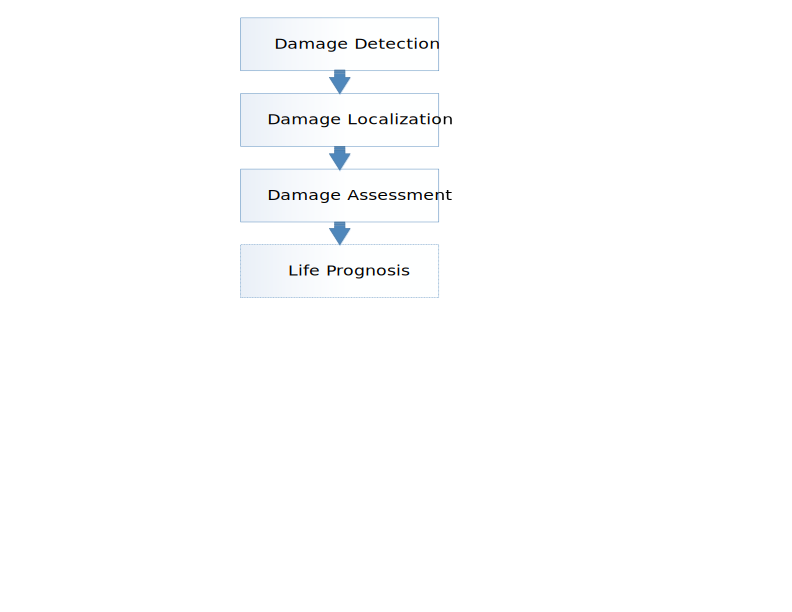
\includegraphics[width=0.5\textwidth]{fig1.1.png}
	\end{center}
	\caption{Four major levels of SHM} 
	\label{fig:fig1.1}
\end{figure}

According to these levels, damage detection level provides a qualitative explanation that the damage may exist, localization level gives an indication about the feasible region of the damage, the assessment level indicates the estimation of the severity of damage by giving information regarding the size and type of damage and at last, the evaluation of remaining structural life is provided at prognosis stage. The prognosis level also predicts possible failures or breakdowns. The initial three levels (i.e. detection, localization, and assessment) are usually related to damage identification, signal processing, and modelling features. The last level (i.e. life prognosis) falls into statistical analysis, reliability, fracture mechanics, fatigue analysis, and design assessment fields. Many researchers have comprehensively investigated the prognosis level but currently, there are no commercially available solutions~\cite{stepinski2013advanced, TibaduizaBurgos2020}. 

\section{SHM and Nondestructive Testing/Evaluation (NDT/E)}
%%%%%%%%%%%%%%%%%%%%%%%%%%%%%%%%%%%%%%%%%%%%%%%%%%
SHM allows for global and online monitoring of large structures~\cite{stepinski2013advanced}. Whereas, NDT/E is usually performed by operator locally as an off-line inspection tool. However, it is not essential as NDT/E is also employed being a monitoring tool for in situ formations i.e. rails and pressure vessels. NDT/E is primarily used for severity check and damage characterization when the damage location is already known~\cite{Farrar2007,Farrar2012}.

SHM requires integrating actuators and sensors, computational power, and data transmission in a structure for the purpose of detecting, assessing, localizing, and predicting defects~\cite{stepinski2013advanced, jawaid2018structural}. An SHM system is mostly concerned with online global damage identification in structures. SHM based techniques are commonly implemented in civil engineering and aerospace structures~\cite{stepinski2013advanced, jawaid2018structural}. 

NDT/E systems are often bounded to single-point measurements while SHM techniques support the online monitoring of large structures and can also perform localization of defects~\cite{stepinski2013advanced}. With new sensors, SHM based methods are suitable for reliable continuous monitoring~\cite{heslehurst2014defects}. For reliable damage detection, the SHM needs more state-of-the-art signal processing than classical NDT/E techniques~\cite{stepinski2013advanced}.

The main difference between SHM and NDT/E systems can be observed from the hardware architecture. In an SHM system, actuators and sensors are integrated with or molded into the structure, while there is no integration involved with the structure in the case of NDT/E. NDT/E is an external system with an independent set of actuators and sensors~\cite{stepinski2013advanced}.
Most of the NDT/E techniques require component disassembly especially for those components that are inaccessible which results in interruption of the daily operation of the structural systems leading to downtime which consequently results in an increase in operational costs. In an effort to improve the integrity of structures, SHM technology has been introduced for the monitoring of civil, mechanical, and aerospace structures~\cite{gopalakrishnan2011computational}.  
NDT/E systems are usually costly, labor-intensive, and time-consuming. Most of the NDT/E techniques depend firmly on the expertise and skills of the operator. Skilled judgment and peculiar experience are required for NDT/E based techniques~\cite{jawaid2018structural}. Furthermore, safety precautions are also essential for most of the NDT/E methods. Nowadays, SHM is becoming more significant in different engineering disciplines such as civil, mechanical, and aerospace. NDT/E techniques are localized in nature whereas SHM deals from a wider perspective. NDT/E demands preceding information of the damage location whereas there is no such provision in SHM. SHM is a more reliable and modified variant of NDT/E~\cite{jawaid2018structural}. SHM can lessen costs and manage a decent level of safety regarding the performance conditions particularly for complex structures~\cite{Balageas2010}. SHM is adopted extensively by the aerospace community, particularly for the aging of aircraft situations~\cite{chang2002introduction}. Technology is gradually progressing toward continuous monitoring and a more enduring attachment, and hence toward SHM. More affordable and smaller sensors must be taken into account in the process of shifting from NDT/E to SHM.

\section{Advantages of SHM}
%%%%%%%%%%%%%%%%%%%%%%%%%%%%%%%%%%%%%%%%%%%%%%%%%%
Many industries want to detect defects in their products and manufacturing structures at the earliest feasible time. These industries carry out some form of SHM for such detection~\cite{Farrar2007, Farrar2012}. The main aim of the SHM system is to maintain information on the state of the inspected structure for the purpose of finding structural defects before they reach critical levels. It also helps in providing adequate information for condition-based maintenance~\cite{Farrar2007}.

The SHM is an efficient approach for the regular monitoring of roads, bridges, skyscrapers, mechanical, civil, and aerospace structures. The new methods and technological developments are being employed in the SHM. The principal benefits of the employment of SHM include longer life spans, increased safety, detection of early risks, and cost-efficiency~\cite{Farrar2012, Crane2017}. Public safety is greatly improved with the use of new SHM methods~\cite{jawaid2018structural}. Regular monitoring and analysis assist in identifying design flaws. SHM is also helpful in recognizing environmental factors that may not have been taken into consideration throughout the construction process. Emergency maintenance and a continual preventative of different structures aids to improve their longevity~\cite{jawaid2018structural}. Another main advantage of SHM is that it greatly reduces short and long-term structural maintenance costs. Furthermore, structural integrity maintenance for a longer span of time lessens overall costs related to rebuilding and demolition~\cite{Lamonaca2018}. 

SHM offers an automatic inspection method for reducing unessential maintenance tasks~\cite{Guemes2020a}. SHM is used as a tool in various industries for preventing unexpected damage which yields vital advantages to the industries. SHM improves the safety and functionality of structures. SHM is useful in the timely warning of impending failures~\cite{TibaduizaBurgos2020, jawaid2018structural}.

In an SHM system, data is gathered on realistic performance, which is very useful for designing improved structures for the future. SHM can ensure safety and avoid the failure of the structure which in turn will save uncountable human losses due to accidents~\cite{jawaid2018structural}. In conventional systems, a considerable number of structures undergo regular assessment and maintenance for the purpose of ensuring the structural stability of the system. This number can easily be reduced by implementing an SHM system which will indicate the healthy structure to be unnecessary for the inspection~\cite{jawaid2018structural}.

\section{Basic Elements of an SHM System}
%%%%%%%%%%%%%%%%%%%%%%%%%%%%%%%%%%%%%%%%%%%%%%%%%%
A typical SHM system is composed of three basic elements: (i) A network of actuators and sensors, most likely smart materials, which are permanently connected to the structure. This perspective of SHM makes it different from conventional NDT/E techniques and it is mandatory for executing automated inspections. This step involves observation of the structure from arrays of sensors using regular sampled response measurements, storing the measured data, and transmitting data to the control center. (ii) On-board information administration and computing equipment. A large number of sensors are continuously producing a huge volume of data for processing in real-time. Computational power and data transmission are employed within a structure for the purpose of detecting, localizing, assessing, and predicting defects which can produce structure impairment immediately or later in the future. (iii) Algorithms that examine collected data from the structure with the recently obtained data. Algorithms also determine a damage index and then notify about the existence, position, type, and size of the damage~\cite{stepinski2013advanced, Guemes2020a, lee2008overview, Crane2017}.

For monitoring of possible changes in the structures, all SHM systems need a proper sensor network. The sensitivity of the SHM techniques is usually linked with better interaction between the sensors and the structure. Therefore, it is essential to choose suitable sensors to be installed. During the implementation of a network of sensors in an SHM system, the information for obtaining defect identification, the material of the structure to examine, and the variables to measure are considered. The next stage is data acquisition. In this stage, the signals produced by each sensor are obtained. The characteristics of SHM systems such as mobility, scalability, and costs are considered. The data collected by the SHM can be influenced by sensor configuration, environmental and operational noise, or any other event. Many of these obstacles need to be resolved before executing any analysis on the produced information for generalizing the methods applied for recognition, identification, or classification. This level is associated with preprocessing or signal conditioning. It can be accomplished with the use of hardware accessories, software algorithms, or both. At last, data analysis tools are used for determining the presence of defects in the instrumented structure and for characterizing the possible source of the damage~\cite{TibaduizaBurgos2020,Crane2017}.

\section{Classification of SHM Methods}
%%%%%%%%%%%%%%%%%%%%%%%%%%%%%%%%%%%%%%%%%%%%%%%%%%
Damage detection techniques for SHM may be categorized into two major classes based on the type of information to be used: Local and Global methods~\cite{lee2008overview, stepinski2013advanced}. 

Local techniques monitor a tiny part of the structure surrounded by sensors using measurements of structural response~\cite{lee2008overview, stepinski2013advanced}. Comparative Vacuum Monitoring (CVM) and Electromechanical Impedance (EMI) are normally considered as local SHM techniques~\cite{Guemes2020a, liang1997coupled, Fiborek2018}.
\newline Global techniques are executed when global motion is induced in the structure during its operation. Vibration-based methods are one of the examples of this class. Global methods are helpful when local damage has an influence on the behavior of the global structure in terms of space and time~\cite{lee2008overview, stepinski2013advanced}. 
As opposed to local methods, global methods have many benefits: 
\newline i) The whole structure can be measured with these methods by using a sparse sensor network.
\newline ii) It is not necessary to locate sensors near the damage.
\newline iii) Only a little information about the critical region is enough. 
Global SHM techniques have also some limitations: 
\newline i) The wavelength of vibrations is nearly equivalent to the dimension of the component or structure, therefore, these methods have relatively low sensitivity to small defects. 
\newline ii) Usually these methods are quite expensive~\cite{ stepinski2013advanced}.

Although the damage size and location are roughly estimated with global methods, it can be successfully utilized for damage detection. The relationship between defects of structures and structural vibration is used in the health assessment~\cite{stepinski2013advanced,Worden2007}. 

Recently, three types of SHM techniques have been successively developed: (1)  SHM based on vibrations~\cite{MMaia}; (2) Electromechanical Impedance (EMI) based SHM~\cite{Fiborek2018}; and (3) Guided wave-based SHM~\cite{Mei2019,Tian2015,Park2014,Sikdar2019,Girolamo2018,Rogge2013,Kudela2018}. Vibration-based SHM techniques detect damage by measuring vibration signals on structures. These techniques identify local defects by detecting changes in modal shapes, natural frequencies, or dynamic responses. EMI based techniques identify changes in structures by measuring the EMI of a PZT transducer, which is connected to (or embedded into) the monitored structure. Guided Waves (GWs) are elastic waves that are propagating along a determined path by the structure boundaries. GWs and the applications of GWs in SHM are explained in the next section.

\section{Guided Wave Based SHM}
%%%%%%%%%%%%%%%%%%%%%%%%%%%%%%%%%%%%%%%%%%%%%%%%%%
\subsection{Guided Waves}

GWs are of huge concern for NDT/E and SHM of engineering structures such as rails, aircraft components, and oil and gas pipelines. Developing a GWs based technique needs attentive understanding obtained over-analysis and modelling of mode-damage interaction and wave propagation because of the dispersion and multimodal character of these waves~\cite{Lugovtsova2019}. These techniques have several benefits: (1) A relatively short wavelength provide plentiful interaction of the GWs and relatively small defects; (2) These waves have very high excitation frequency, therefore, low-frequency ambient influence can be filtered out; (3)  GWs can propagate comparatively longer distances inside the structure under investigation; (4) It provides better sensitivity to various types of defects and the extent of the monitored area.

Velocity, scattering, attenuation, and mode conversion are some of the features which are used for indicating changes in structural dynamics~\cite{Wang2020,Mitra2016}. In these techniques, an actuator is used which travels through the structure for generating the waves. Signals are received by the transducers at one or multiple locations which are then analyzed for the identification of defects. In GWs, damage can be detected and monitored with a very small number of transducers~\cite{Munian2018}. In many GWs based SHM techniques, collections of actuators/sensors are adjusted on a plate which not only identifies the existence of defects but also localize the defects~\cite{Farrar2012}.

In the GWs based SHM techniques, usually, an array of PZTs is utilized for sensing and excitation of signals. It provides the ability of online monitoring and the permanent integration of modifications in GWs propagation. However, the problem of applying an array composed of some PZTs for the localization of defects is that the resolution of the imaging of defects may be very low. Whereas, applying a highly dense arrangement of PZTs is also not feasible. This problem can be solved by adopting Scanning Laser Doppler Vibrometry (SLDV). SLDV is capable of measuring GWs under a very dense grid of points over the surface of a large specimen. This combination of signals is known as full wavefield~\cite{Wandowski2011,Radzienski2019}.

\subsection{Lamb Waves}

Lamb wave is a form of ultrasonic guided waves which propagates in plate-like structures~\cite{Lamb1917}. Lamb waves interrogation of structures is an appealing SHM technique for damage detection and monitoring. Lamb waves can travel longer distances with minimum dispersion. These waves are also highly sensitive towards detecting small defects. Damage in structures using Lamb waves can be evaluated by analyzing modifications in the propagation of Lamb waves considering backward and forward scattering~\cite{Hameed2019b}. These waves give more enhanced information about the presence, size, type, location, and severity of damage than frequency response techniques~\cite{Kessler2002}. Both internal and external defects in large monitoring structures can be inspected with Lamb waves. Due to these reasons, Lamb waves have been established to be highly suitable for damage detection in plate-like structures~\cite{Kudela2018a}. For the generation and detection of Lamb waves, the Lead Zirconate Titanate (PZT) are mostly used~\cite{Journal}. Both contact and non-contact type of transducers such as air-coupled ultrasonic transducers can be employed for the generation of Lamb waves. Sophisticated signal-processing techniques are used for the processing of the dynamic response signals received by PZT transducers~\cite{Hameed2019a,Su2004}. 

These waves are guided by the free surfaces of plates. The wavelength of Lamb waves is similar or larger than the thickness of the plate. These waves couple shear and longitudinal waves within a plate. To use Lamb waves for SHM techniques, it is beneficial to possess a waveform which is efficiently recognizable before and after the propagation through the plate. The frequency dependency of wave speed in Lamb waves makes these waves dispersive. However, varying frequency components are propagating at diverse velocities inside the plate. A narrow-band frequency helps to reduce the unwanted dispersive nature of Lamb waves~\cite{Kessler2002}. By choosing a proper driving frequency, the response of the input signal is recorded at receiving sensors with minimal interference~\cite{Farrar2012}. 

The propagation of Lamb waves can be categorized into either Symmetric ($S_0$) or Antisymmetric ($A_0$) modes. The $A_0$ mode of Lamb waves is quite valuable for damage identification. The wavelength and wave velocity of $A_0$ mode is relatively smaller than $S_0$ mode. The smaller wavelength of $A_0$ mode is very helpful because for interacting with the damage, the half wavelength of a chosen wave mode must be smaller or similar to the size of the damage. $A_0$ modes can efficiently be generated by the surface mounted transducers~\cite{Ricci2016}.  

The main problem of Lamb waves is that it is an active technique. It needs a regular supply of voltage and function generating signals. The resulting data of Lamb waves is more complicated than many other techniques. Therefore, the interpretation of these signals is also very difficult~\cite{Kessler2002}.

Despite an extensive number of research efforts, Lamb waves based real engineering applications are still limited. This is mainly because of the complexity of the propagation of these waves, i.e. dispersion, possible reflections from boundaries, multimodal nature, and also more structural features which generate a wave field which is laborious to analyse~\cite{stepinski2013advanced}.

\section{Types of Sensors used in GWs based SHM}
%%%%%%%%%%%%%%%%%%%%%%%%%%%%%%%%%%%%%%%%%%%%%%%%%%
In the last few years, the structural engineering community is increasingly implementing sensor networks for SHM purposes of monitoring structures. For an SHM system, it is essential to acquire a proper assessment of a system dynamic response. There are several different types of sensors and data retrieval methods that can be implemented in the SHM. The sensors used in an SHM system are application-specific~\cite{Farrar2012}.

SHM sensing and data acquisition system consists of some or all of the below-mentioned elements:
\newline 1. Transducers that are responsible for converting changes in the domain variable of interest i.e. temperature, strain, or acceleration to changes in an electrical signal i.e. voltage, resistance, or impedance.
\newline 2. Actuators which are responsible for applying a recommended information to the system i.e. a PZT transducer attached to the surface of a structure.
\newline 3. Analogue-to-Digital (A/D) converters that are responsible for converting analogue electrical signals into digital signals which can be processed later on digital hardware. When an SHM system is using actuators, a Digital-to-Analogue (D/A) converter is also required for converting a designated digital excitation signal to an analogue voltage which is useful for controlling the actuator~\cite{Farrar2012}. 

Damage detection for an SHM needs the employment of an arrangement of sensors with the primary function of capturing data which can be employed for determining the state of the monitored structure. Many SHM systems employ elastic wave signals which are produced by an actuator. The inspection methods depend on the transducer type used for inspection and also the type of propagating signals over the structure. The transducers employed in the SHM system should be light and small in size for the purpose of integration into the structure without any considerable impact on its behavior. Due to the improved implementation of SHM methods, a lot of new sensors have been developed. These new sensors are very helpful in improving the ability of detection, characterization, and localization of defects in an SHM system. These advancements in sensors strive to reduce the weight and power consumption of the system. In addition, it also helps in resolving installation problems, and for improving data analysis and operation facilities. The subsequent sections illustrate some of the various types of sensors used in SHM systems. These sensors can be adapted for the inspection of both composite and metallic structures. Sensors can be categorized on the basis of physical variable which they sense or on the principle of transduction on which they are based. Some of these sensors, their advantages, disadvantages, and the inspected variable are shown in Tab 1.1~\cite{Farrar2012,TibaduizaBurgos2020}.

\subsection{Piezoelectric Sensors}
Piezoelectric materials are made of polymers and ceramic. Piezoelectric transducers are a category of devices that satisfy most of the demands of SHM. Piezoelectric transducers are lightweight, less expensive, small in size, consumes a low amount of power, and is able to generate frequency response in a wider region. Some other advantages of piezoelectric sensors are: these sensors can be assembled in various forms, such as circular, rectangular, and longitudinal. PZT transducers can be used for rapid and in situ SHM. These transducers can easily be arranged as a arrays of sensors in order to record multipoint measurements on or under the surface of the monitored structure. However, the methods utilizing these transducers sometimes needs a high amount of data points and the baseline signal for the purpose of comparison with the damaged signal for authentic damage estimation~\cite{Farrar2012,Hameed2019}.
These transducers are mostly used for sensing and generation of guided waves. With these transducers, it is easy to measure wave propagation and acquire information about various damage types, such as corrosion or delamination~\cite{TibaduizaBurgos2020,Mitra2016}.

\subsection{Fiber Optics}
Fiber Optics sensors are employed in those situations where high precision and immunity to electromagnetic-interference is required. These sensors are useful for measuring temperature, acceleration, vibrations, pressure, rotation, deformation, shifting, and material concentrations~\cite{TibaduizaBurgos2020}. For deformation analyses, Fiber Optics Sensors (FOS) and Fiber Bragg Grating (FBG) sensors are mostly used. FOS are less costly, usually contain multimode fibers and auto-compensate for temperature changes. Whereas, FBG sensors are employed as discriminating filters of any wavelength~\cite{TibaduizaBurgos2020}. 

\subsection{Microelectromechanical Systems (MEMS)}
Miniaturization techniques are used in the construction of this type of sensors and it combines several kinds of transducers. These sensors are very beneficial in the case of costs of maintenance and implementation. MEMS sensors have some additional attractive characteristics too, such as their smaller size or capability of easy connectivity with a wireless sensor network. It is also desirable to find MEMS sensors that utilize inductive, optical effects, capacitive, or piezoelectric. In addition, actuators can also be included. Generally, MEMS is composed of a mixture of multiple varieties of sensors. These sensors are adopted for measuring the magnitude of distinct variables i.e. angular velocity (gyroscopes), deformation, displacement, and acceleration. This type of sensors provides high sensitivity, the integration of communication systems, the determination of multiple variables, and responses at lower frequencies. Recently, the use of MEMS sensors has significantly increased due to the mentioned factors~\cite{Farrar2012, TibaduizaBurgos2020}.

\subsection{Scanning Laser Doppler Vibrometer (SLDV)}
Laser Doppler Vibrometer (LDV) works on the principles of the Doppler shift.  LDV is highly applicable for the measurement of the out-of-plane surface velocities. LDV measures these velocities with high precision including non-contact mode during guided wave propagation~\cite{Mitra2016}. LDV sensing systems have been widely employed for the sensing of guided waves and more specifically for Lamb waves~\cite{Mitra2016}. 

Generally, an LDV based sensing system contains a laser head that drives a laser beam and then records the reflected beam of the vibrating surface. A demodulator is used for transforming the information of the reflected beam into velocity measurements, and then a controller is used to deflect the optical mirrors for the purpose of precise adjustment of the laser beam. A simpler LDV sensing system contains a single head that can offer only a single point measurement. The Scanning LDV (SLDV) is capable of recording and measuring the vibrations at various points on a predetermined grid. SLDV provides high resolution, rapid, and precise imaging of the wave response of a structure in a non-contact way~\cite{Mitra2016}. SLDV enables measurement of full wavefield of a structure rather than single-point measurements usually obtained through conventional sensors. SLDV is useful for measuring the velocity of the inspected area in points associated with a predefined grid. SLDV based measurements can be combined with adequate signal processing and imaging algorithms for the purpose of damage identification. High resolution based SLVD measurements provides very detailed visualization of different types of multiple defects~\cite{Kudela2015}.

A layout of mirrors is equipped with SLDV which is helpful for changing the angle of measurement beams. The SLDV is also equipped with a camera which is helping for defining a measurement grid precisely on the selected area of the object of interest. Furthermore, a screen of monitor is used for the visualization of the grid. 3D vibrometers are used for providing information of the monitored object in three dimensions which is very helpful in many cases. However, acquiring 3D measurements are more challenging than obtaining 1D measurements because 3D measurements need an added alignment of the three laser beams~\cite{Ostachowicz2014}.

Recently, notable progress has been carried out in the measurement techniques such as shearographic interferometry and SLDV. These techniques allow analysis of a full wavefield of elastic waves. The advancement in these techniques initiated new opportunities for the various types of damage detection problems in structures~\cite{Mitra2016}.

SLDV have some limitations too, which are: (1) The inspected object surface has to be characterised by proper reflectivity. In other case, the acquired signal-to-noise ratio is low. (2) For a specified time, the measurements can only be performed at one point in space. (3) SLDV is very expensive. (4) The measurements need to be repeated many times for full field Lamb wave registration at a dense grid of points~\cite{Ostachowicz2014}.
(5) High resolution measurement of SLDV takes much time and needs a large amount of hard drive space.

\begin{table}[h]
	\centering
	\caption{Details of various types of sensors used in SHM}
	\begin{adjustbox}{width=\textwidth = {!},center}
\begin{tabular}{ccccc}
	\hline
	\textbf{Sensor Type}                                                                                                 & \textbf{Technology}          & \textbf{Variable to Measure}               & \textbf{Advantages}                                                                  & \textbf{Disadvantages}                                            \\ \hline
	\multirow{5}{*}{Piezoelectric}                                                                                       & PZT                          & Acceleration                               & Low Cost                                                                             & Thermal Sensitivity                                               \\ \cline{2-5} 
	& PVDF                         & Deformation                                & Low Price                                                                            & Aging                                                             \\ \cline{2-5} 
	& \multirow{3}{*}{P(VDF-TrFE)} & Corrosion                                  & Integration Possibilities                                                            &                                                                   \\ \cline{3-5} 
	&                              & Vibration                                  & \multicolumn{1}{l}{}                                                                 & \multicolumn{1}{l}{}                                              \\ \cline{3-5} 
	&                              & Displacement                               & \multicolumn{1}{l}{}                                                                 & \multicolumn{1}{l}{}                                              \\ \hline
	\multirow{6}{*}{Fiber Optics}                                                                                        & \multirow{5}{*}{FOS}         & Rotation                                   & \begin{tabular}[c]{@{}c@{}}Electromagnetic Interference\\  Immunity\end{tabular}     &                                                                   \\ \cline{3-5} 
	&                              & Acceleration                               &                                                                                      & Fragility                                                         \\ \cline{3-5} 
	&                              & Vibrations                                 & Integration Possibilities                                                            & \multicolumn{1}{l}{}                                              \\ \cline{3-5} 
	&                              & Pressure                                   & \multicolumn{1}{l}{}                                                                 & \multicolumn{1}{l}{}                                              \\ \cline{3-5} 
	&                              & Shifting                                   & \multicolumn{1}{l}{}                                                                 & \multicolumn{1}{l}{}                                              \\ \cline{2-5} 
	& FBG                          & Deformation                                & High precision                                                                       & High price                                                        \\ \hline
	\multicolumn{1}{l}{\multirow{5}{*}{\begin{tabular}[c]{@{}l@{}}Microelectromechanical\\ Systems (MEMS)\end{tabular}}} & MEMS                         & Deformation                                & Low cost                                                                             & \begin{tabular}[c]{@{}c@{}}High-frequency\\ Response\end{tabular} \\ \cline{2-5} 
	\multicolumn{1}{l}{}                                                                                                 & \multirow{4}{*}{NEMS}        & Deformation                                & \begin{tabular}[c]{@{}c@{}}Different Kinds of\\ Sensors and\\ Variables\end{tabular} & \multicolumn{1}{l}{}                                              \\ \cline{3-5} 
	\multicolumn{1}{l}{}                                                                                                 &                              & Displacement                               & Wireless Connection                                                                  & \multicolumn{1}{l}{}                                              \\ \cline{3-5} 
	\multicolumn{1}{l}{}                                                                                                 &                              & \multicolumn{1}{l}{Acceleration Gyrometer} & Small Size                                                                           & Fragility                                                         \\ \cline{3-5} 
	\multicolumn{1}{l}{}                                                                                                 &                              & Shifting                                   & \multicolumn{1}{l}{}                                                                 & \multicolumn{1}{l}{}                                              \\ \hline
\end{tabular}
\end{adjustbox}
\end{table}

\section{GWs based SHM in Composite Structures}
%%%%%%%%%%%%%%%%%%%%%%%%%%%%%%%%%%%%%%%%%%%%%%%%%%
In recent years, various industries are progressively employing composite structures for achieving the desired performance in a wide area of applications~\cite{Hameed2019b}. The use of composite structures is growing rapidly due to its simple structure, high specific strength, lightweight, and many other desired mechanical properties~\cite{Radzienski2019}. 

Maintenance is required for the composite materials because of less frequent and complex material failures in them. 
The state of a structure in which the structure fails to provide adequate output is termed as the failure of the composites. This failure in composite structures depends upon many quantitative and qualitative factors such as structural stiffness of the composite, the strength of the structures, resistance to corrosion, resistance to impact, fatigue due to loading and unloading cycles, resistance toward lightning and thunderstorms, and yield capacity of the composite~\cite{Rahul2018}. Different forms of damage can occur in composite materials such as matrix cracking, debonding, delamination, and fiber breakage~\cite{Yu2019,Fakih2019}. Composite structures are very sensitive to impact loads. Even a low-intensity and the low-velocity impact can commence matrix cracks in composites. The matrix cracks in composites then lead to delamination which is one of the most common susceptible defects in composite structures. Delamination can grow and badly affect the structural integrity and mechanical properties of the composites~\cite{Munian2018}. 

In recent decades, many researchers have developed numerous intelligent and computational based SHM techniques for composite structures. Eddy currents (electromagnetic testing), acoustic emissions, optical methods, ultrasonic inspection, vibration analysis, thermography, radiography, and Lamb waves are extensively used damage detecting techniques in composite structures~\cite{Rahul2018}. Guided Lamb waves are broadly recognized as one of the most promising tools for significant identification of defects in composite structures~\cite{stepinski2013advanced,Ricci2016}. GWs based SHM techniques have been broadly applied for detecting numerous types of defects in composite structures, including debonding~\cite{Sikdar2019}, delamination~\cite{Tian2015,Park2014}, and impact damage~\cite{Girolamo2018,Rogge2013,Kudela2018}. Lamb waves based SHM techniques are commonly applied for damage detection in composite structures. 

Lamb waves based detection, identification, and localization of damage for composite structures have extensively been studied in the literature. Yang et al.~\cite{Yang2019} evaluated the size, location, and shape of damage with Lamb waves by using PZT wafer transducers in composite materials. Hameed et al.~\cite{Hameed2019b} developed an efficient damage detection technique by introducing quantitative size estimation and transverse damage localization for composite materials with the use of Lamb waves. Li et al.~\cite{Li2012} developed a technique on the basis of the second harmonic Lamb waves propagation for assessing the thermal fatigue defects in composite materials. Zak et al.~\cite{Zak2012} used laser scanning vibrometry for experimental measurements for defects detection in metal and thin-walled composite materials with the use of guided Lamb waves. They applied the spectral finite element method for numerical investigations. Fakih et al.~\cite{Fakih2019} proposed a Lamb wave-based technique for the detection, localization, and assessment of the severity for barely visible indentation damage in composite structures. Toyama and Takatsubo~\cite{Toyama2004} used an Acoustic Emission (AE) transducer and Angle Beam Transducer (ABT) for the detection of impact damage in composite laminates using $S_0$ mode of Lamb waves. Rauter et al.~\cite{Rauter2015} developed an impact damage detection method for composite structures on the basis of nonlinear Lamb waves.

\section{Conclusion}
%%%%%%%%%%%%%%%%%%%%%%%%%%%%%%%%%%%%%%%%%%%%%%%%%%
In this chapter, the need for carrying out SHM in various industries, and the main levels of SHM along with the functionalities of every level are elaborated. Firstly, the damage is detected then the location of the damage is identified after that the size and type of damage are estimated and in the end, the remaining life of the structure is evaluated. The interrelation and major differences between SHM and NDT/E techniques are also demonstrated. Furthermore, the intentions and benefits of carrying out SHM are presented. Different types of SHM techniques and the basic components of SHM are described. Various kinds of sensors applied for implementing SHM techniques are explained. PZT based transducers are usually preferred over fiber optics and MEMS sensors due to their smaller size and low cost. The use of guided waves, Lamb waves, and SLDV in SHM are also explained. Guided Lamb waves are usually preferred over vibrations and EMI for implementing SHM techniques due to its longer propagation distances and suitability for distinguishing smaller defects. Furthermore, various types of guided wave-based damage detection, localization, and assessment techniques implemented in composite materials are described. In the end, major challenges of SHM are discussed. Implementation of SHM techniques is challenging due to lack of available data, sensor failures, high cost, and accuracy of damage identification in real-world scenarios.

\section*{Acknowledgements}

The research was funded by the Polish National Science Center under grant agreement no 2018/31/B/ST8/00454.
%%%%%%%%%%%%%%%%%%%%%%%%%%%%%%%%%%%%%%%%%%%%%%%%%%
%\subsection{Description}
%%%%%%%%%%%%%%%%%%%%%%%%%%%%%%%%%%%%%%%%%%%%%%%%%%
%text
%%%%%%%%%%%%%%%%%%%%%%%%%%%%%%%%%%%%%%%%%%%%%%%%%%

%\begin{figure} [h!]
%	\begin{center}
		%\includegraphics[width=14cm]{Graphics/bc.jpg}
%	\end{center}
%	\caption{Figure caption.} 
%	\label{fig:bc}
%\end{figure}

%%%%%%%%%%%%%%%%%%%%%%%%%%%%%%%%%%%%%%%%%%%%%%%%%%

%\begin{table}[h]
%\centering
%	\caption{Table caption}
%	\begin{tabular}{cccc}
%		\hline
%	\textbf{a}	& \textbf{x} & \textbf{y} & \textbf{z} \\
%		\hline
%		-50 & -0.289 & -0.289 & -0.598\\ 
%		-40 & -0.248 & -0.248 & -0.512\\ 
%		\hline 
%	\end{tabular} 
%	\label{tab:xyz}
%\end{table}
%%%%%%%%%%%%%%%%%%%%%%%%%%%%%%%%%%%%%%%%%%%%%%%%%%

%The scheme of experimental setup is shown in Fig.~\ref{fig:bc}.  
%The values are collected in Tab.~\ref{tab:xyz}.


%The details are described in a book~~\cite{udd2011fiber}. 

%Similar case was analysed~\cite{Badrinarayanan2017a} by Hill et al.
%Additional information:
%\begin{itemize}
%\item fonts Times New Roman, 11pt
%\item keep figures separately in greyscale with resolution 600 dpi (publisher requirement)
%\item 20-30 pages
%\item Bibliography~\cite references in the order of citations within the text
%\end{itemize}

\bibliography{report} % 
%bibliography data in report.bib
\bibliographystyle{unsrt}
% makes bibtex use spiebib.bst


%%%%%%%%%%%%%%%%%%%%%%%%%%%%%%%%%%%%%%%%%%%%%%%%%%
\end{document}
%%%%%%%%%%%%%%%%%%%%%%%%%%%%%%%%%%%%%%%%%%%%%%%%%%
